%%
%% This is file `example.tex',
%% generated with the docstrip utility.
%%
%% The original source files were:
%%
%% coppe.dtx  (with options: `example')
%% 
%% This is a sample monograph which illustrates the use of `coppe' document
%% class and `coppe-unsrt' BibTeX style.
%% 
%% \CheckSum{1391}
%% \CharacterTable
%%  {Upper-case    \A\B\C\D\E\F\G\H\I\J\K\L\M\N\O\P\Q\R\S\T\U\V\W\X\Y\Z
%%   Lower-case    \a\b\c\d\e\f\g\h\i\j\k\l\m\n\o\p\q\r\s\t\u\v\w\x\y\z
%%   Digits        \0\1\2\3\4\5\6\7\8\9
%%   Exclamation   \!     Double quote  \"     Hash (number) \#
%%   Dollar        \$     Percent       \%     Ampersand     \&
%%   Acute accent  \'     Left paren    \(     Right paren   \)
%%   Asterisk      \*     Plus          \+     Comma         \,
%%   Minus         \-     Point         \.     Solidus       \/
%%   Colon         \:     Semicolon     \;     Less than     \<
%%   Equals        \=     Greater than  \>     Question mark \?
%%   Commercial at \@     Left bracket  \[     Backslash     \\
%%   Right bracket \]     Circumflex    \^     Underscore    \_
%%   Grave accent  \`     Left brace    \{     Vertical bar  \|
%%   Right brace   \}     Tilde         \~}
%%
\documentclass[msc,
pdftex,
%doublespacing,
numbers]{coppe}
\usepackage[T1]{fontenc}
\usepackage{amsmath,amssymb}
\usepackage{lmodern}
\usepackage[utf8]{inputenc}

\makelosymbols
\makeloabbreviations

\begin{document}
  \title{Utilização de uma metaheurística hibrida para solução do problema de construção de trilhos de aeronaves }
  \foreigntitle{Using a hybrid metaheuristic for solving the aircraft rotation problem}
 \author{Alexander}{de Almeida Pinto}
  \advisor{Prof.}{Nome do Primeiro Orientador}{Sobrenome}{D.Sc.}
  \advisor{Prof.}{Nome do Segundo Orientador}{Sobrenome}{Ph.D.}
  \advisor{Prof.}{Nome do Terceiro Orientador}{Sobrenome}{D.Sc.}

  \examiner{Prof.}{Nome do Primeiro Examinador Sobrenome}{D.Sc.}
  \examiner{Prof.}{Nome do Segundo Examinador Sobrenome}{Ph.D.}
  \examiner{Prof.}{Nome do Terceiro Examinador Sobrenome}{D.Sc.}
  \examiner{Prof.}{Nome do Quarto Examinador Sobrenome}{Ph.D.}
  \examiner{Prof.}{Nome do Quinto Examinador Sobrenome}{Ph.D.}
  \department{SDI}
  \date{1}{2011}

  \keyword{Transporte}
  \keyword{PCTA}
  \keyword{Metaheurística}
  \keyword{Método Exato}
  \keyword{GRASP}
  \keyword{Rotas de Aeronáves}
  
  \maketitle

  \frontmatter
  
  \dedication{A minha família e amigos cuja valia é imensurável.}

  \chapter*{Agradecimentos}

  Gostaria de agradecer a todos que fizeram 

  \begin{abstract}

  Apresenta-se, nesta tese, ...

  \end{abstract}

  \begin{foreignabstract}

  In this work, we present ...

  \end{foreignabstract}

\tableofcontents
\listoffigures
%\listoftables
\printloabbreviations
\printlosymbols


  \mainmatter
  \chapter{Introdução}

  A indústria aeronáutica tem sido uma rica fonte de problemas no que diz respeito à pesquisa operacional, sendo confrontados diariamente com problemas de alto grau de complexidade e que possuem uma natureza combinatória explosiva. Por causa da dificuldade que é inerente a essa classe de problemas a qualidade das soluções obtidas manualmente são muito aquém da melhor solução possível. 
  
Nos dias de hoje, no entanto, com o avanço da tecnologia e o aumento da competitividade desenvolver soluções com melhor qualidade acaba se tornando um fator decisivo para a permanência no mercado, tornando-se então necessário a obtenção de soluções de forma mais rápida, mais barata e utilizando menos recursos. Outra  característica que reforça a necessidade da obtenção de melhores soluções é o aumento do tamanho e da complexidade das instâncias trabalhadas. A partir desse cenário pode-se perceber a necessidade de utilização de técnicas de otimização, na literatura tem se observado um crescimento no número de trabalhos que se utilizam de metaheurísticas como método de resolução.
  
As metaheurísticas podem ser definidas como um conjunto de procedimentos de caráter geral, com capacidade de guiar o procedimento de busca, tornando-o capaz de escapar de ótimos locais. Elas têm como objetivo, encontrar uma solução tão próxima quanto possível da solução ótima do problema com baixo esforço computacional.
  
Em geral, as metaheurísticas são bastante utilizadas na resolução de problemas de otimização. Esses problemas, também conhecidos como problemas NP-difíceis\abbrev{NP}{Non-Polinomial}, podem ser definidos como um conjunto de problemas para os quais ainda não existe um algoritmo que os resolvam de forma exata e em tempo polinomial \citep{maritan}.
  
Para esses tipos de problemas o uso de métodos exatos é bastante restrito, uma vez que o esforço computacional para encontrar uma solução exata em instâncias reais é consideravelmente alto. No entanto, na prática, é suficiente encontrar uma solução próxima do ótimo global. 

A literatura pesquisada mostra uma grande quantidade de tentativas de resolver o problema utilizando modelagens matemáticas, que apesar de garantir a solução ótima não se mostra viável para resolver grandes instâncias. \citep{clarke97}. Alguns trabalhos mostram a similaridade desse problema com o problema do caixeiro viajante assimétrico \cite{clarke97}. E outros resolvem uma parte do problema utilizando metaheurísticas.\citep{arguelo1007}
%#############################################
%{\large >>>> Descrever em que tem se baseado a solução desse problema na literatura <<<<}
%#############################################

Os principais problemas relacionados dizem respeito ao planejamento envolvendo a criação de linhas de trabalho tanto para as aeronaves quanto para a tripulação. O objetivo costuma ser a minimização dos custos operacionais ou a maximização dos rendimentos. Custos operacionais consiste nos custos envolvidos com combustíveis, óleo, taxas de aterrissagem e a perda de rendimentos com a utilização de aeronaves com menos assentos do que a demanda de passageiros, porém fatores como bem estar dos passageiros também podem ser levados em consideração.

	Os problemas de planejamento que envolvem as aeronaves mais estudados na literatura são o Fleet Assigment e o Aircraft Rotation. E os que envolvem a tripulação são conhecidos como Crew Pairing e o Crew Scheduling.

	O problema Fleet Assigment trata da alocação da frota, ou seja, é determinado o tipo de equipamento a ser utilizado em cada voo [Pimentel, 2005]. O problema Aircraft Rotation será descrito mais adiante. O problema Crew Pairing visa obter o melhor conjunto de pairings \footnote{Pairing é o conjunto de voos que pode ser guiados por uma tripulação sem que seja violadas quaisquer regras da legislação vigente e que ao final do ultimo voo o tripulante esteja de volta a sua cidade base. }  tal que cada voo seja coberto por pelo menos um pairing. Gastos com alojamentos, alimentação, transporte em terra e deadheads \footnote{Deadhead é o voo que o tripulante viaja sem trabalhara com a finalidade de transporte para outra localidade normalmente para sua base ou para suprir uma nova demanda. } devem ser levados em consideração. O problema Crew Scheduling tem o objetivo de atribuir os pairings a tripulação disponível na companhia aérea, acrescentando as atividades de solo tais como call \footnote{Call é o tempo que a tripulação tem para se apresentar a companhia aérea antes de iniciar de fato seu turno de trabalho.} , Stand-by duties \footnote{Stand-by duties são turnos em que o tripulante fica a disposição da companhia aérea afim de suprir possíveis eventualidades.}  e dias de descanso. O objetivo dessa etapa é fazer uma distribuição da forma mais justa possível, tentando balancear a quantidade de trabalho (horas a serem voadas) entre os tripulantes, e também tentar cumprir todas as solicitações da tripulação em relação a preferência dos dias de descanso e das tarefas a serem realizadas.

	Após as designação da frota de aeronaves ao conjunto de voos existentes segue-se o problema de construção de trilhos de aeronaves (PCTA) \abbrev{PCTA}{Problema de Construção de Trilhos de Aeronaves} que também é conhecido na literatura como Aircraft Rotation Problem (ARP) \abbrev{ARP}{Aircraft Rotation Problem}. O PCTA é um dos principais problemas presentes na industria da aviação. No PCTA o objetivo é a construção, para cada uma das frotas da companhia (e para os voos a elas alocados), de sequências encadeadas de vôos que possam ser operados por uma única aeronave \citep{abiliolivro}. Cada uma dessas sequências recebe o nome de trilho.
 
	O sequenciamento dos voos pode ocorrer de 4 formas distintas aqui denominado de arcos. Os arcos do tipo 1 permitem a ligação de voos sem a utilização de atrasos e/ou reposicionamentos. Os arcos do tipo 2 utilizam atrasos mas não o reposicionamento. Os arcos do tipo 3 permitem o sequenciamento com a utilização de um voo de reposicionamento mas sem inserir atraso em nenhum dos voos envolvidos. Os arcos do tipo 4 utilizam-se de atrasos e de um voo de reposicionamento para fazer a ligação entre dois voos.
 
	Para resolver o PCTA, devemos estar cientes de algumas restrições que envolvem tempo e espaço. Por exemplo, um avião não pode partir antes da chegada do vôo que lhe antecede, nem de um local diferente da cidade de destino deste mesmo vôo. Há também a restrição de que um vôo deve permanecer em solo, entre conexões, por um período de tempo que seja suficiente para fazer a troca de passageiros e abastecimento da aeronave e quando for o caso para a troca de tripulação, esse tempo varia de acordo com o aeroporto. O PCTA sofre um grande quantidade de restrições sendo as mais importantes as temporais e geográficas.
 
	Vale ressaltar que na resolução do PCTA deve-se levar em consideração as particularidades especificas de cada companhia aérea como o número de aviões disponíveis na frota, o atraso máximo permitido nos voos, a quantidade máxima de voos que podem sofrer atraso, o número máximo de voos que podem ser cancelados, o número máximo de voos de reposicionamento que podem ser criados entre outros.
 
	Outro aspecto importante diz respeito às restrições de manutenção. Sabe-se que um avião deve ter checagens periódicas. Oportunidades de realizar essas tarefas ocorrem apenas em algumas conexões potencialmente disponíveis. Como consequência, uma sequência de voos deve ser construída de forma que essas restrições não sejam violadas. A fim de incorporar essas restrições facilmente ao nosso framework, assumimos que as rotações são designadas a tipos não específicos de aeronave. Dessa forma, se uma aeronave tem necessidade de manutenção, um vôo especial é criado com origem e destino na base de manutenção escolhida. O tempo desse vôo é exatamente o tempo de manutenção [Pontes, 2003].
 
	De uma maneira geral, o principal objetivo do PCTA é a minimização do número de trilhos seguido da minimização do custo total dos trilhos gerados. Esse custo pode envolver diversos componentes, sendo o tempo médio diário de utilização das aeronaves um dos mais importantes \citep{abiliolivro}.
 
	Abaixo na Figura \ref{arpexample} temos dois exemplos de montagem de trilhos feitas a partir de um conjunto fictícios de voos. Cada caixinha laranja e azul representa um voo, onde a parte laranja representa o tempo de solo que cada voo deve obedecer e a azul seria o tempo de voo da cidade de origem para a cidade de destino. As letras A, B, C, D, E representam as cidades e a linha pontilhada indica o tempo de inicio e de termino de cada voo.

\begin{figure}[ht]
	\centering
	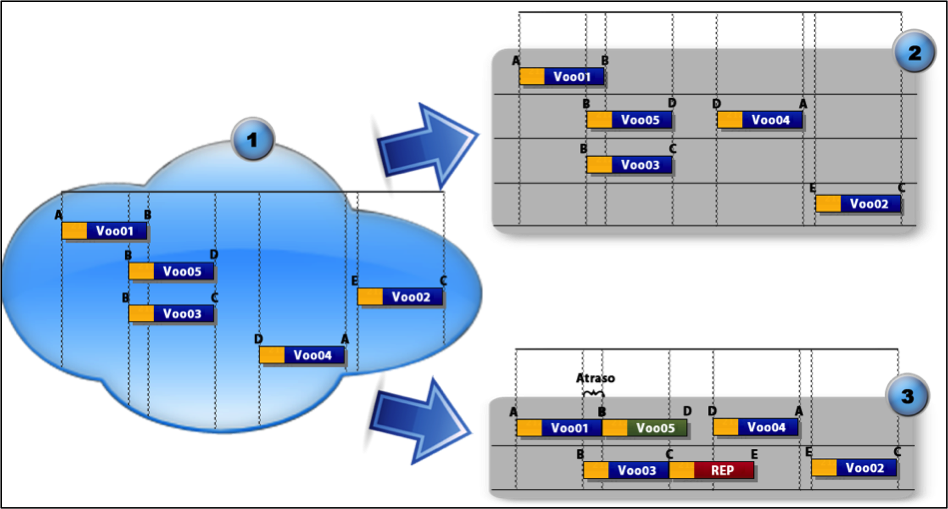
\includegraphics[scale=0.9]{./img/arpexample}
	\caption{Construção de Trilhos de Aeronaves}
	\label{arpexample}
\end{figure}

A parte 1 da Figura \ref{arpexample} representa os voos da companhia que ainda não foram cobertos por nenhuma aeronave e nas partes 2 e 3 são demonstrado duas formas de organizar esses voos em trilhos. 

	Na parte 2 temos a melhor forma possível de se organizar os voos da parte 1 utilizando apenas os arcos do tipo 1, ou seja sem a utilização de atrasos ou de voos de reposicionamento. Dessa forma se consegue uma formação com 4 trilhos.

	Na parte 3 temos a melhor forma de organizar os voos utilizando todos os arcos e um atraso máximo equivalente a um tempo de solo. Dessa forma se consegue uma formação com apenas 2 trilhos.

	Pode-se verificar que a utilização de diferentes tipos de arcos pode proporcionar uma melhora significativa  no número de trilhos. Porém essa abordagem faz com que o número de soluções possíveis tenha uma cardinalidade muito superior a utilização de arcos apenas do tipo 1 que por si só já gera uma quantidade de soluções bem elevada, por isso os arcos devem ser utilizados de forma controlada. 

	Nesse trabalho propomos o desenvolvimento de um método híbrido baseados em metaheurísticas e em programação para resolução do PCTA. O método proposto procura combinar a eficiência computacional das metaheurísticas com a rápida convergência dos métodos exatos. Além disso ficou constatado pelo levantamento da literatura acerca do PCTA que se tem uma falta de instâncias sobre o problema que permitam uma melhor comparação dos resultados obtidos, logo também propomos um conjunto de instância baseado em uma instância real da TAM, com vários tamanhos e complexidades. 

%#############################################
{\large	>>>> Fazer uma breve descrição de programação linear, maiores detalhes serão dados na fundamentação teórica. <<<<	}
%#############################################

\section {Objetivos do trabalho}

Tendo em vista os aspectos apresentados, o objetivo principal dessa proposta de trabalho consiste no desenvolvimento de um método híbrido baseado em metaheurísticas e programação linear para a resolução do problema construção de trilhos de aeronaves (PCTA). O método proposto irá se basear em uma metaheurísticas, afim de explorar a eficiência computacional, e irá ser combinada com etapas de refinamentos composta por métodos exatos para acelerar a convergência e adicionalmente fugir de mínimos locais.

Além disso irá ser proposto um conjunto de instâncias baseados em uma instância real da TAM variando em complexidade e tamanho, essas instâncias irão permitir uma melhor comparação desse trabalho com outros.

\section {Organização da proposta }

A dissertação está estruturada da seguinte forma:

\begin{itemize}

\item Capítulo 1: Apresenta a motivação e as vantagens de resolver o PCTA utilizando metaheurísticas e programação linear e enfatiza a importância desse problema na indústria aeronáutica.  Ao final os objetivos do trabalho são descritos.

\item Capítulo 2: Apresenta a fundamentação sobre a otimização, metaheurísticas e programação linear. Na seção referente à otimização além da descrição serão discutidos algumas heurísticas  construtivas e de refinamento. A seção referente às metaheurísticas irá iniciar com uma descrição seguida pela descrição das metaheurísticas utilizadas no trabalho, como o Greedy Randomized Adaptive Search Procedure (GRASP) e o Iterated Local Search (ILS). E a seção referente a programação linear vai descrever como o algoritmo simplex consegue resolver problemas modelados matematicamente. Ao final da fundamentação teórica será feita uma revisão dos principais trabalhos descritos na literatura relacionada ao presente trabalho.

\item Capítulo 3: Mostra como foi obtida a malha da companhia de transporte aéreo TAM e como foi gerado as instâncias que são utilizadas no trabalho.

\item Capítulo 4: Descreve o método proposto nesse trabalho, os parâmetros, as restrições e a modelagem matemática utilizada.

\item Capítulo 5: Apresenta alguns resultados preliminares que já foram obtidos com o método que é utilizado atualmente.

\item Capítulo 6: Apresenta as referencias bibliográficas que deram suporte a confecção do presente trabalho.

\item No final é apresentado o cronograma de trabalho proposto durante os 24 meses de mestrado. 
\end{itemize}


  \chapter{Fundamentação Teórica}

  Nesse capítulo será feita a fundamentação dos principais assuntos presente nesse trabalho: a heurística construtiva, a heurística de refinamento, as metaheurísticas e a programação linear. Nas seções seguintes serão descritas os aspectos teóricos e os principais métodos relacionados a esse trabalho.

	\section{Heurísticas Construtivas}
		As técnicas de resolução heurísticas se utilizam de processos intuitivos afim de obter uma boa solução, a um custo computacional aceitável, ou seja não garante a otimalidade de um problema. O objetivo é obter em um tempo reduzido uma solução tão próxima quanto possível do ótimo global. 
		
		Uma heurística é dita construtiva quando a construção da solução se dá elemento por elemento. A forma de escolha dos elementos variam de acordo com a estratégia e a função de avaliação adotada, essa escolha deve levar em consideração o benefício da inserção de cada elemento para a solução final, escolhendo sempre o \emph{melhor} elemento em cada passo.
		A Figura \ref{heuristicaconstrutiva} mostra o pseudocódigo para a construção de uma solução inicial para um problema de otimização que utiliza uma função gulosa \emph{g(.)}. Nesta figura, \emph{$t_{melhor}$} indica o membro do conjunto de elementos candidatos com o valor mais favorável da função de avaliação \emph{g}, isto é, aquele que possui o menor valor de \emph{g} no caso de o problema ser de minimização ou o maior valor de \emph{g} no caso de o problema ser de maximização.
		
\begin{figure}[ht]
	\centering
	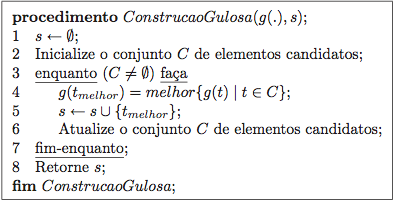
\includegraphics[scale=0.7]{./img/heuristicaconstrutiva}
	\caption{Heurística de construção gulosa de uma solução inicial}
	\label{heuristicaconstrutiva}
\end{figure}

Uma outra forma de obter uma solução inicial é escolhendo os elementos candidatos aleatoriamente. Isto é, a cada passo, o elemento a ser inserido na solução é aleatoriamente selecionado dentre o conjunto de elementos candidatos ainda não selecionados. A grande vantagem desta metodologia reside na simplicidade de implementação. Segundo testes empíricos , a desvantagem é baixa qualidade em média da solução final. Essa técnica é recomendada quando a característica do problema torna mais fácil o refinamento do que a construção de uma solução \citep{notasmarcone}. 

A Figura \ref{construcaoaleatoria} mostra o pseudocódigo para a construção de uma solução inicial aleatória para um problema de otimização.

\begin{figure}[ht]
	\centering
	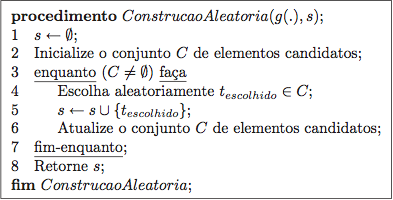
\includegraphics[scale=0.7]{./img/construcaoaleatoria}
	\caption{Heurística de construção aleatória de uma solução inicial}
	\label{construcaoaleatoria}
\end{figure}

Para melhores resultados essa etapa deve ser seguida de um refinamento.

		
	\section{Heurísticas de Refinamento}
	
		As heurísticas 	de refinamento são técnicas que se utilizam de uma solução inicial qualquer (que pode ter sido gerada por uma heurística construtiva ou então gerada aleatoriamente) e aplica a noção de vizinhança com finalidade de modificar essa solução caminhando, a cada iteração, de vizinho para vizinho transformando-as em outras que estejam presentes em sua vizinhança de acordo com a definição adotada. Os \emph{movimentos} são as modificações que são aplicadas na solução inicial \emph{s} para que ela se transforme em outra \emph{s`}.
		
		A definição de vizinhança é bem importante, partindo de uma solução \emph{s} do espaço deve ser possível atingir qualquer outra solução em um número finito de passos, utilizando um determinado tipo de movimento. Por exemplo, considere o problema do cacheiro viajante em que \textbf{... (Finalizar exemplo do cacheiro viajante)}
		
		Diversos problemas combinatórios tem como característica uma alta dificuldade na obtenção de soluções viáveis. Nesses casos pode se tornar interessante a geração de soluções vizinhas mesmo que elas não sejam viáveis, através da relaxação de algumas restrições e a aplicação de uma penalização a essas soluções. 
		
		Em geral é vantajoso a utilização de uma heurística de refinamento que pode permitir tanto a obtenção de mínimos locais da solução inicial bem como escapar de mínimos locais. Apesar dessas vantagens, dependendo das características dos algoritmos utilizados pode se ter uma quantidade grande de vizinhos a serem percorridos, por isso algumas técnicas podem ser utilizadas.
		
	
		\subsection{Método da primeira descida/subida}
		
		\subsection{Método da primeira melhora}
		\subsection{Método randômico de descida/subida}
		\subsection{Método randômico não ascendente/descendente}
		
\section{Metaheurística}
	\subsection{GRASP}
	\subsection{ILS}
\section{Programação Linear}
\section{Revisão da literatura}
		
		O Trabalho de Argüello e Bard \citep{arguelo1007} (1997) resolve a parte de reconstrução de uma solução do PCTA que tenha sido corrompida por causa de atrasos e impedimentos de voos que ocorrem durante a execução de uma malha. Ele resolve esse problema utilizando a metaheurística GRASP, gerando vizinhos da solução atual de forma sucessiva até obter uma que seja considerada suficientemente boa.
		
		Mercier e Soumis \cite{mercier2007} (2007) resolveram o PCTA em conjunto com o problema de escala de tripulantes pois Cordeau et al. \cite{cordeau2001}, Klabjan et al. \cite{klabjan2002} e Cohn e Barnhart \cite{mainville2003} mostraram que a resolução desses problema de forma integrada pode gerar soluções que são significantemente melhor que as geradas de forma sequencial. O Modelo matemático proposto em CITAR AQUI foi adaptado para auxiliar na geração da nossa solução. 
		
%GRASPs have been used to find high quality solutions to a variety of logistics and combi- natorial optimization problems including maintenance base %planning (Feo and Bard, 1989), machine scheduling (Feo et al., 1991), and number partitioning (Argu ̈ello et al., 1996) to name a few.

  \chapter{Geração das instâncias}
  
  Atualmente existem diversas fontes na qual se podem obter instâncias para problemas de otimização combinatória sendo uma das mais conhecidas a OR-Library \footnote{ pode ser acessado em http://people.brunel.ac.uk/~mastjjb/jeb/info.html} que foi descrito inicialmente descrito em J.E.Beasley \cite{orlibrary} permitindo o acesso a centenas de conjuntos de instâncias a partir da Internet. 
  
Apesar da existência dessas entidades não foi encontrado nenhuma instância que fosse compatível com o problema de construção de trilhos de aeronaves, fazendo-se então necessário a criação de um conjunto de instâncias próprias que além de permitir a conclusão desse presente trabalho ainda servirá como base para futuras propostas.
  
A obtenção de dados foi feita através da seleção manual do conjunto de voos domésticos cobertos pela empresa de transporte aéreo brasileira denominada TAM (http://www.tam.com.br/) que tinham o tempo de partida na segunda feira e se utilizava do equipamento AirBus Industrie A319. A segunda-feira foi identificada como sendo o dia 0 (zero) apenas para permitir sua utilização no algoritmo. Essa instância que foi obtida é composta por X voos e possui uma grande quantidade de ligações entre os Y aeroportos envolvidos tornando o grau de complexidade mais elevado que instâncias com a características hub-and-spoke que é mais comum nas malhas comerciais norte-americanas. Uma malha é considerada como sendo hub-and-spoke quando existe uma grande concentração de vôos em poucos aeroportos como pode ser visto na Figura K.
  
Para se obter um limite inferior dessas instâncias foi feita uma verificação com o algoritmo do Anexo X que permite checar a quantidade mínima de vôos que colidem em uma determinada janela de tempo que é definida pelo atraso máximo permitido. (Pode-se fazer uma formula para explicar esse funcionamento). Essa quantidade é dito como sendo o limite inferior da instância e é garantido que não existe solução com uma melhor quantidade de trilhos que essa sem que nenhum vôo seja excluído.
  
	A TAM tinha disponível nessa época com N aeronaves desse tipo, logo acreditamos que esse é o número de aeronaves que era necessário para atender a todos esses vôos, fazendo com que reduzir essa quantidade de vôos se tornasse um dos objetivos desse trabalho.
  
	Diversas instâncias também foram geradas a partir dessa, variando o número de voos e as características das malhas  com a finalidade de gerar instâncias com um variado grau de complexidade. Essas instâncias podem ser vistas no Anexo N e podem ser solicitadas diretamente com o autor, porém existe a intenção de adicionar esse conjunto de instâncias na OR-Library.
  
	Ainda é necessário a adição de outras instâncias reais para que a validação dos resultados se tornem mais práticos, para isso é necessário a colaboração de empresas de transporte aéreo uma vez que a obtenção desses dados por meios manuais se mostrou demorado e trabalhoso. 
  
  \chapter{Método Proposto}
  \chapter{Resultados preliminares e Discussões}
  \chapter{Conclusões}

  \backmatter
  
  \bibliographystyle{coppe-plain}
  \bibliography{bibliografia}

  \appendix
  %\chapter{Algumas Demonstra{\c c}\~oes}
   \chapter*{Cronograma}
    A seguir temos o cronograma das atividades que foram e que serão desenvolvidas no decorrer do curso de pós graduação.
    
\begin{figure}[ht]

	\centering
	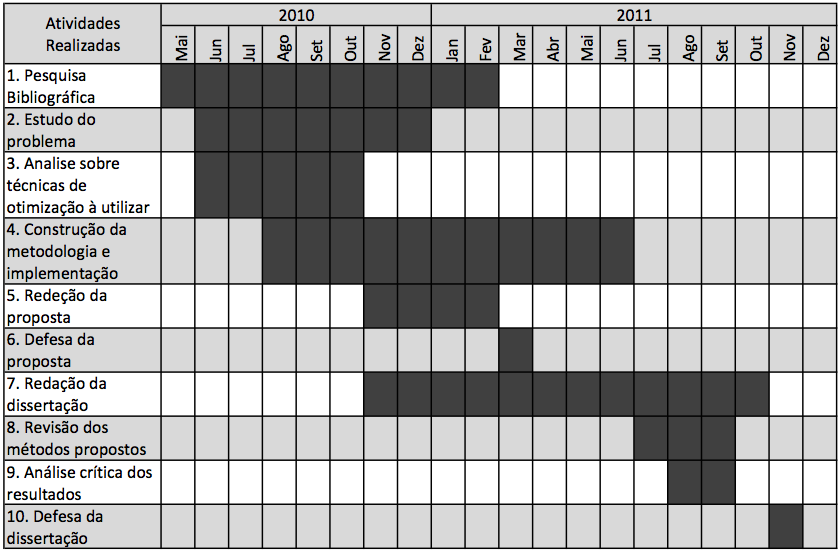
\includegraphics[scale=0.48]{./img/cronograma}
	%\caption{Heurística de construção aleatória de uma solução inicial}
	\label{cronograma}
 \end{figure}
    
Inicialmente foi feito um levantamento bibliográfico sobre o PCTA e outros que são correlatos ou similares a ele, também foi pesquisado sobre metaheurísticas que tiveram bons resultados com esses tipos de problemas. Em seguida foi estudado a possibilidade de integração da metaheurística escolhida com alguma modelagem matemática eficiente. Após isso foi elaborado e implementado o método proposto.

Fica faltando ainda a finalização dessa implementação e a revisão do método proposto, bem como a análise crítica dos resultados. Após essa parte a redação da dissertação para posterior defesa da mesma. O mês de dezembro fica vago para o caso de ocorrer algum imprevisto no decorrer da execução do cronograma.

    

\end{document}


%% 
%%
%% End of file `example.tex'.
